\documentclass[12pt,a4paper]{article}
\usepackage{styles}

\lstset{style=sharpc, tabsize=1}


\author{Alexander van Schie \& Oli Dias}
\title{Gruppenarbeit 1 - Cloud Fundamentals beim Provider}
\begin{document}
\maketitle
\newpage
\tableofcontents
\newpage
\section{Hands-On: Hello (Cloud) World}
\subsection{Installationsanleitung}
Für das Einrichten der Openshift Cloud müssen folgende Schritte durchgeführt werden:
\begin{itemize}
	\item Erstellen eines Accounts unter \url{https://manage.openshift.com/sign_in}
\end{itemize}
\begin{figure}[h]
	\centering
	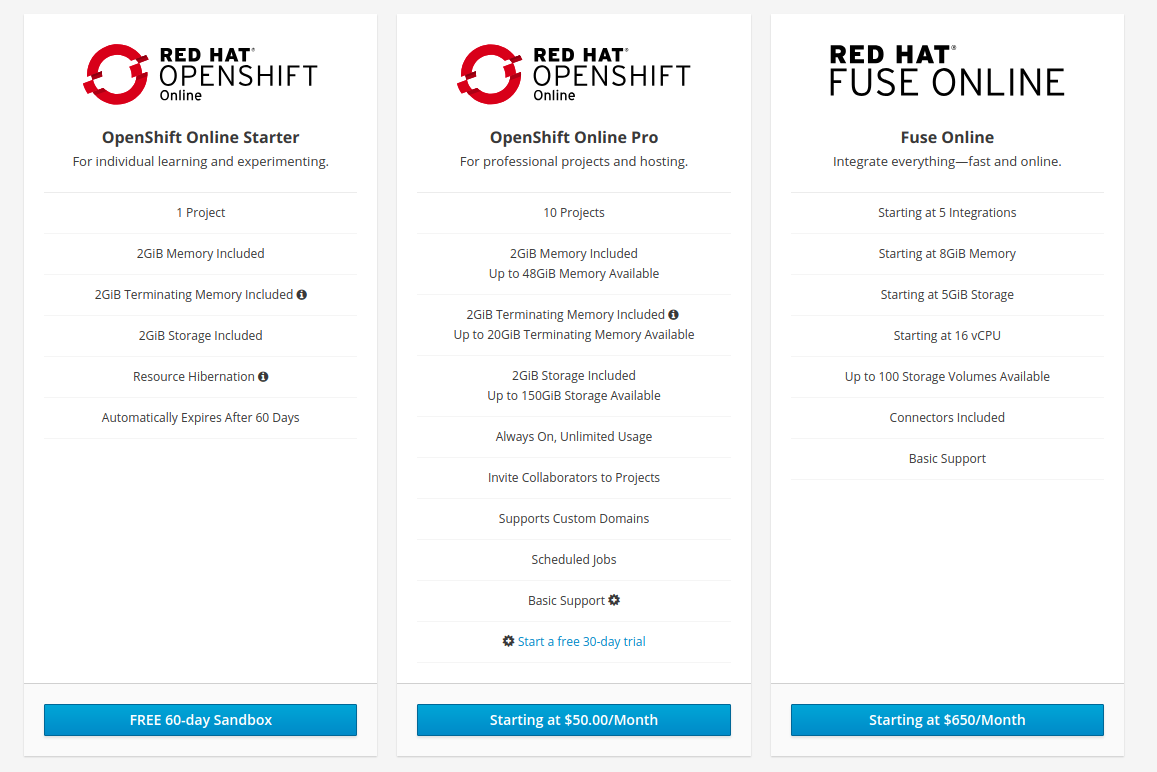
\includegraphics[width=0.7\linewidth]{img/openshift-plan}
	\caption{Gewählter Plan Openshift}
	\label{fig:openshift-plan}
\end{figure}


\begin{figure}[h]
	\centering
	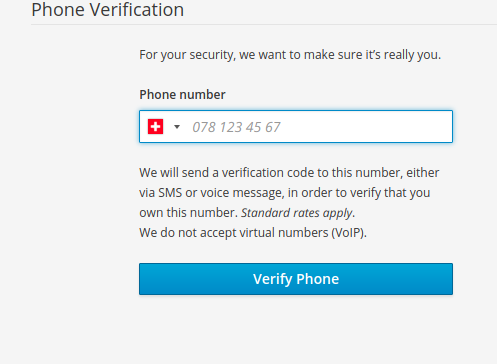
\includegraphics[width=0.7\linewidth]{img/os-phone-validation}
	\caption{Telefon Verifikation}
	\label{fig:os-phone-validation}
\end{figure}

\begin{figure}
	\centering
	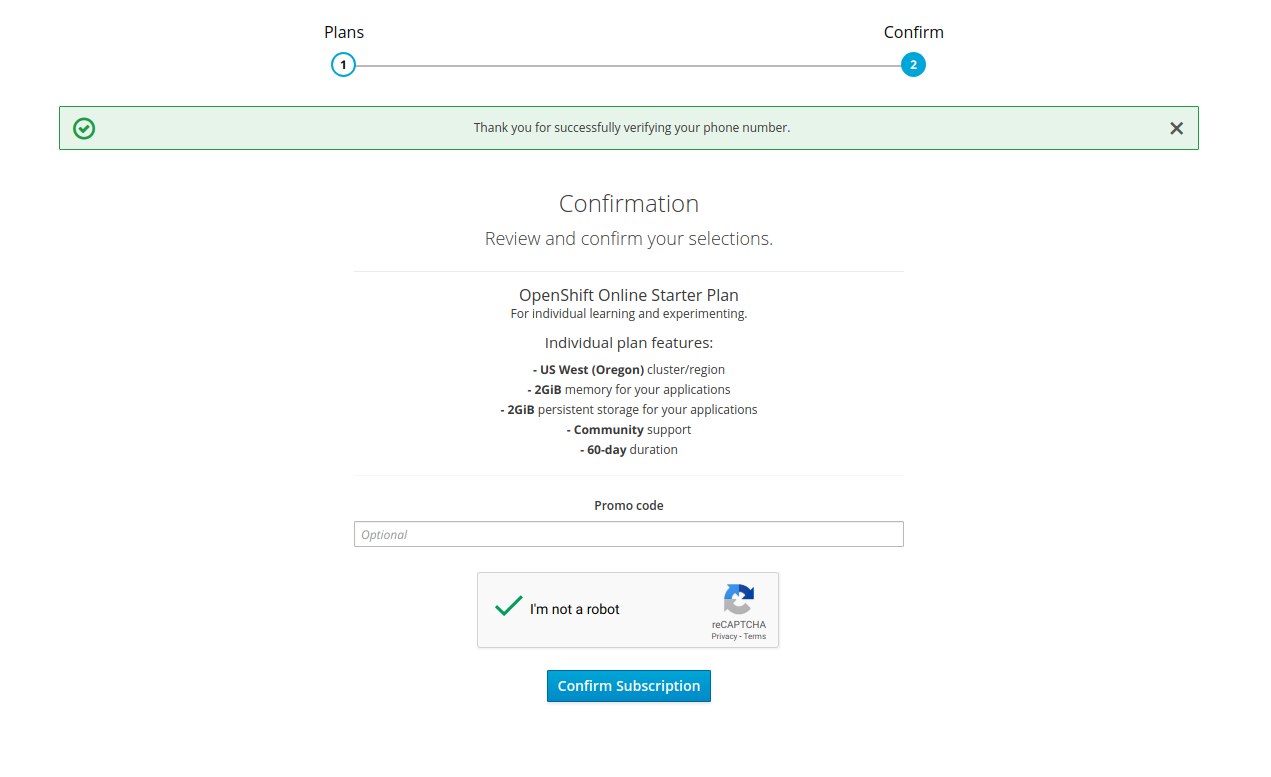
\includegraphics[width=0.7\linewidth]{img/os-overview}
	\caption{Übersicht des abgeschlossenen Plans}
	\label{fig:os-overview}
\end{figure}
Nach kurzer Zeit sollte ein Bestätigungsmail eintreffen, nach welchem die Web Console nun geöffnet werden kann:
\begin{figure}[h]
	\centering
	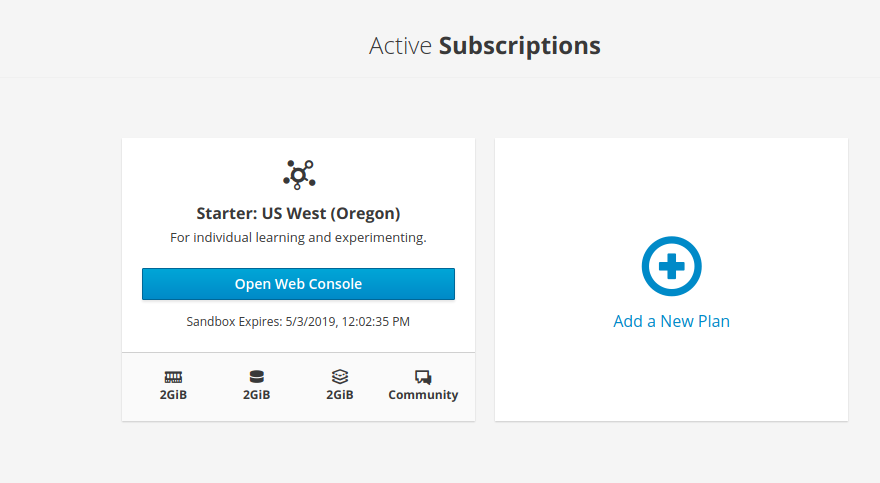
\includegraphics[width=0.7\linewidth]{img/os-web-console}
	\caption{Aktives Abo bei Openshift}
	\label{fig:os-web-console}
\end{figure}

\begin{figure}[h]
	\centering
	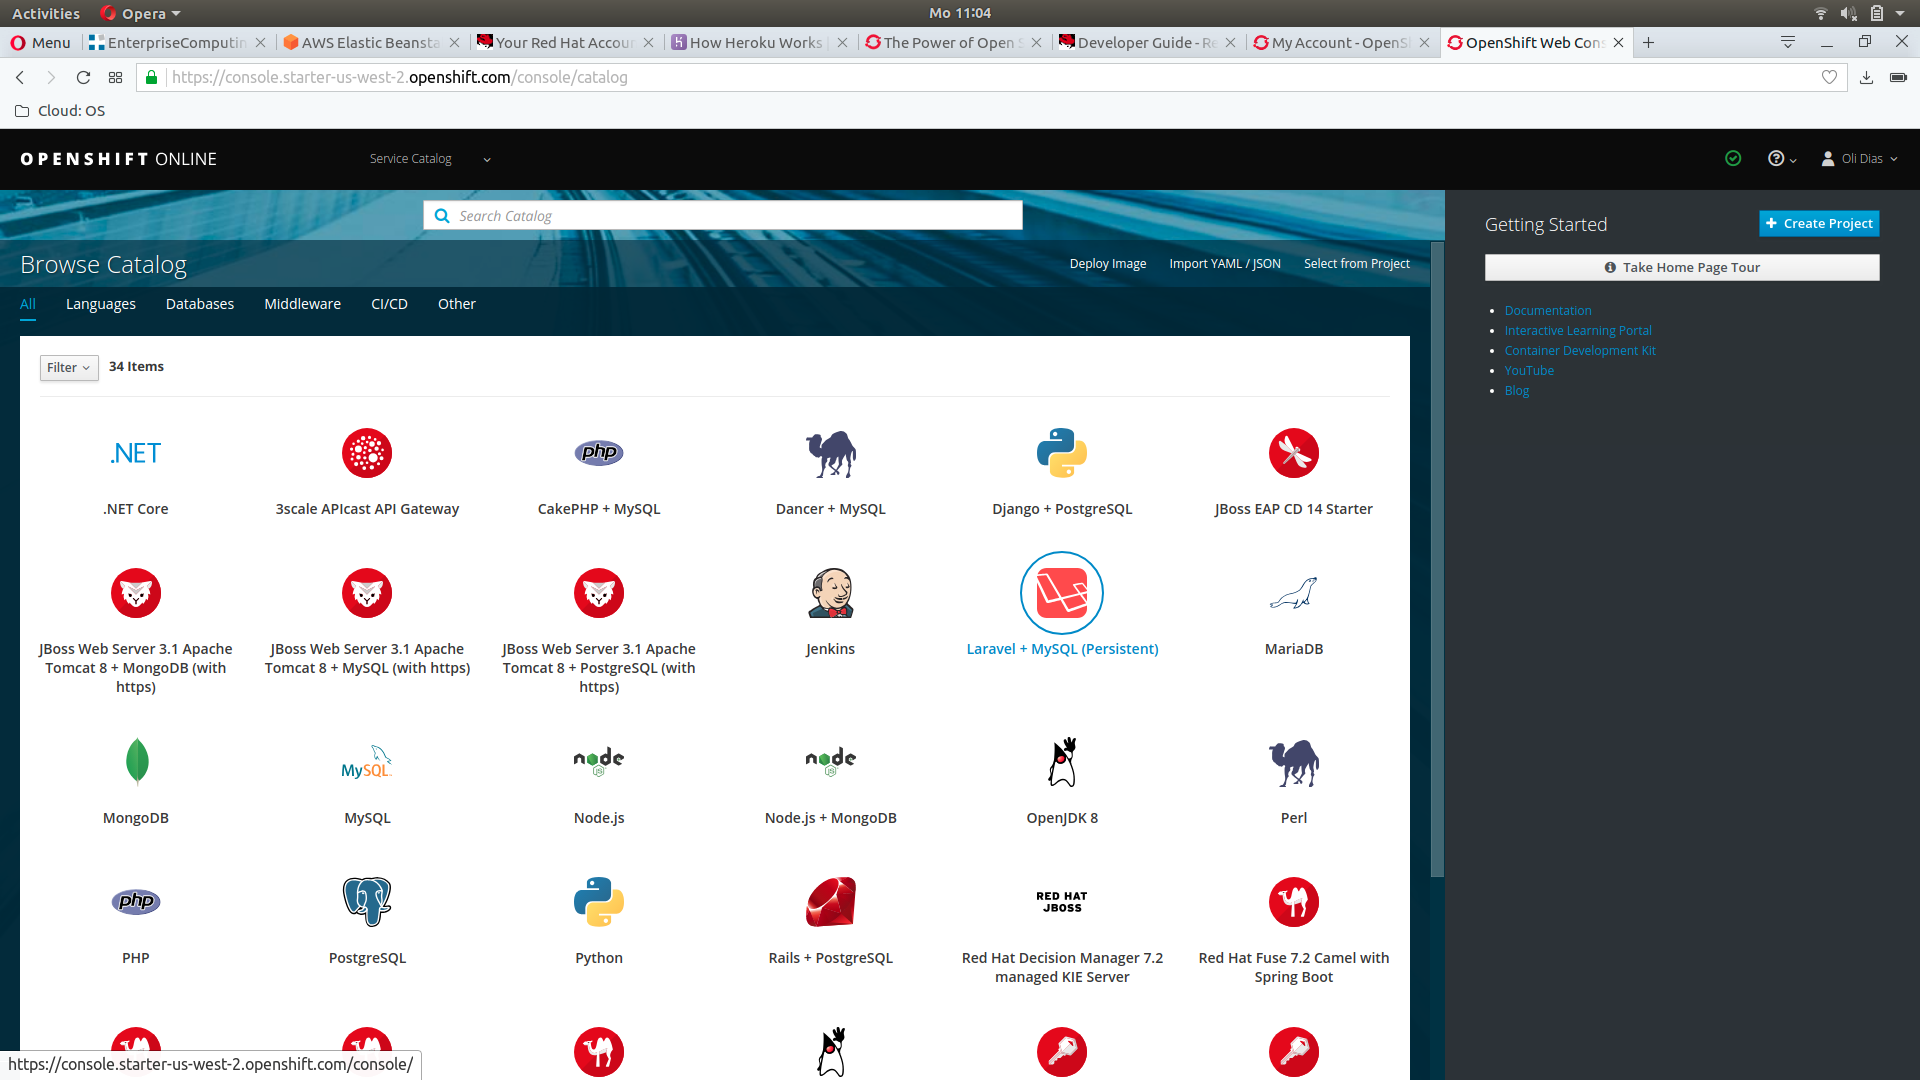
\includegraphics[width=0.7\linewidth]{img/os-overview-catalog}
	\caption{Katalog von Openshift}
	\label{fig:os-overview-catalog}
\end{figure}

\begin{figure}
	\centering
	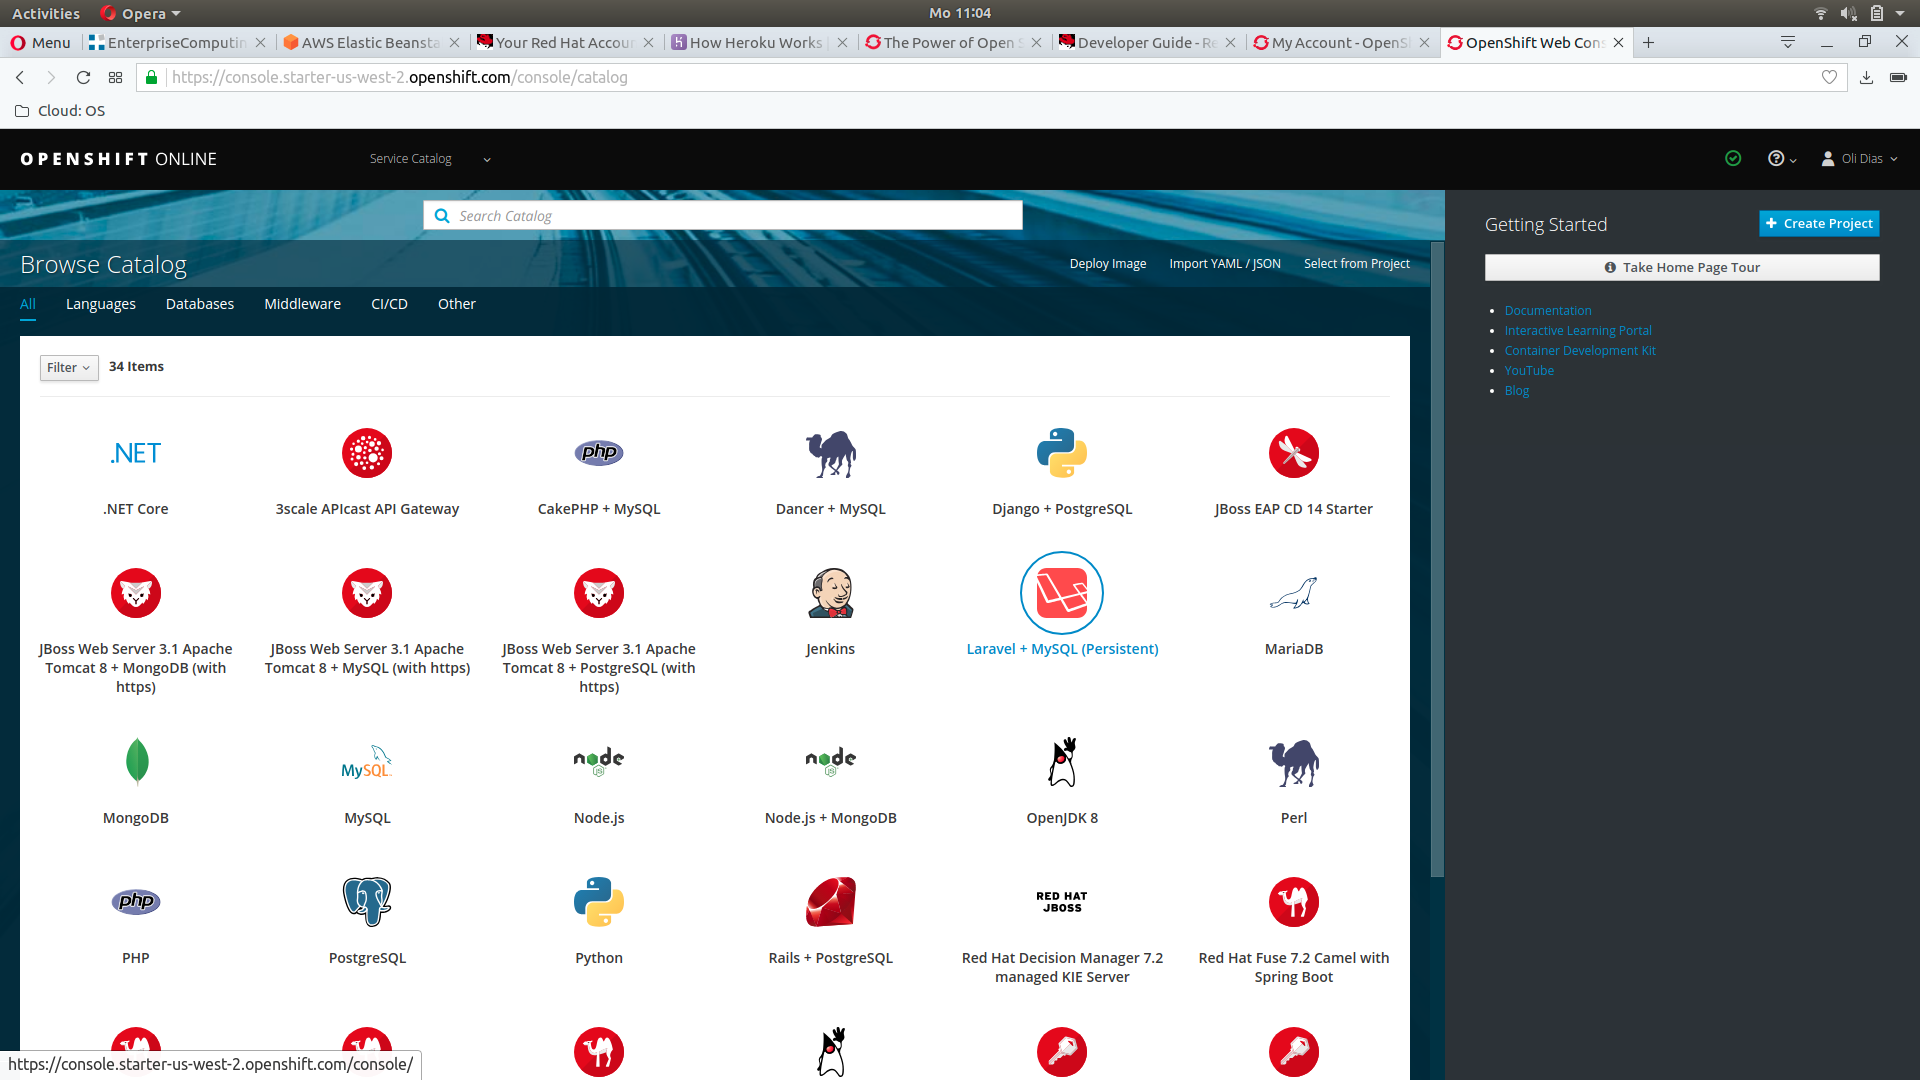
\includegraphics[width=0.7\linewidth]{img/os-new-dotnet}
	\caption{Neues Projekt .Net Core}
	\label{fig:os-new-dotnet}
\end{figure}
Prerequesite: Sicherstellen, dass Git-Repository existiert und sichtbar ist.

\begin{figure}[h]
	\centering
	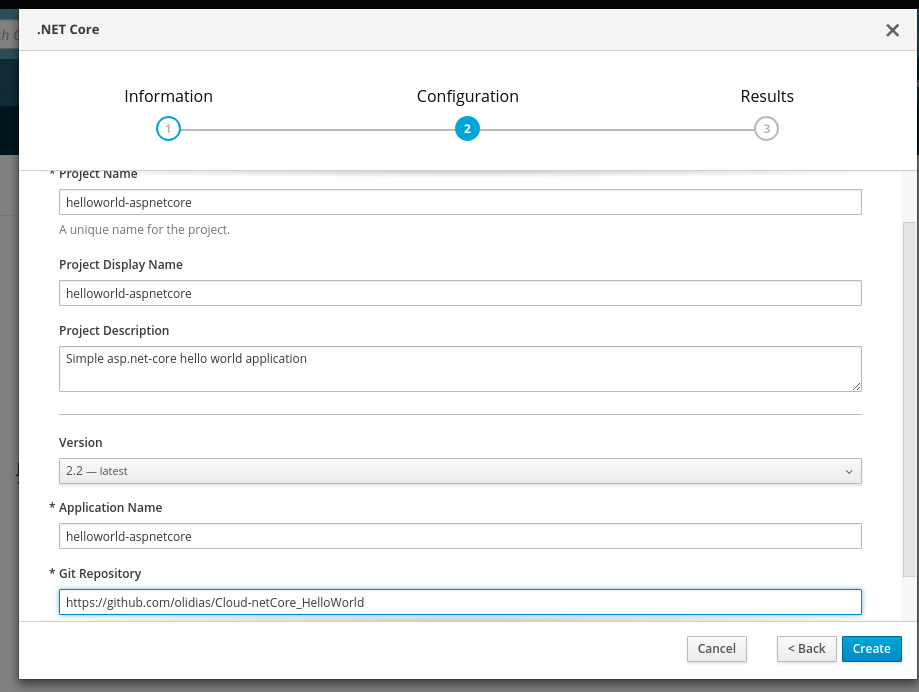
\includegraphics[width=0.7\linewidth]{img/os-new-config}
	\caption{Konfiguration des neuen Projektes}
	\label{fig:os-new-config}
\end{figure}

Sobald das Projekt in Openshift erstellt wurde, startet der Build. 
\begin{figure}[h]
	\centering
	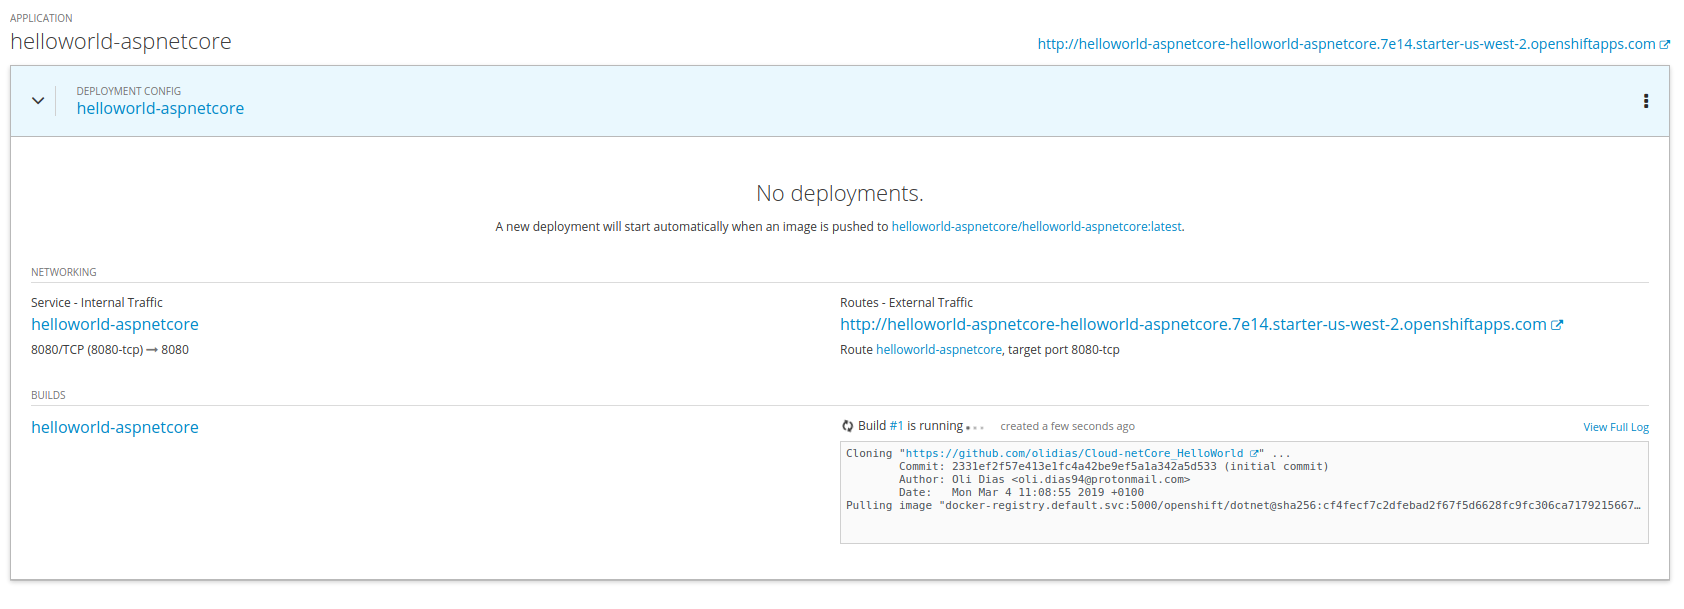
\includegraphics[width=0.7\linewidth]{img/os-building}
	\caption{Builden der .net core Applikation}
	\label{fig:os-building}
\end{figure}
Womöglich schlägt der Build aufgrund von fehlender \texttt{.s2i}-Konfiguration (Source-2-Image) fehl. Um diesen Fehler zu beheben, muss Openshift gesagt werden, wo das dotnet Startup Projekt liegt. Dazu muss ein Ordner und File mit dem Namen \texttt{.s2i/environment} erstellt werden. Dies beinhaltet folgendes:
\begin{lstlisting}[breaklines=true]
DOTNET_STARTUP_PROJECT=HelloWorld-netcore/HelloWorld-netcore.csproj
\end{lstlisting}
Wichtig ist weiter zu beachten, dass die .net Versionen (dotnet sowie NuGet-Pakete) mit denjenigen von Openshift Cloud kompatibel sind. 

War der Build erfolgreich, muss noch das Deployment konfiguriert werden. Dazu kommt ein weiteres File mit dem Namen \texttt{run} ins \texttt{.s2i} Verzeichnis. Darin muss die Applikation noch gestartet werden. Dies funktioniert so:
\begin{lstlisting}
exec dotnet run
\end{lstlisting}
\section{Analyse: OSSM-Definition}

\section{Konzept: Cloud Computing Patterns}

\section{Hands-On: Self Information}

\section{Analyse: Preisrecherche}

\section{Analyse: Preisvergleich eigenes Hosting, IaaS und PaaS}

\end{document}